\chapter{Lecture 23 - ODE Review and Euler's Method for IVPs}
\label{ch:lec23n}
\section{Objectives}
The objectives of this lecture are to:
\begin{itemize}
\item Review some terminology and concepts regarding differential equations
\item Describe Euler's method for 1st order initial value problems (IVPs) and demonstrate convergence behavior
\item Describe and demonstrate the modified Euler's method
\end{itemize}
\setcounter{lstannotation}{0}

\section{Ordinary Differential Equations (ODEs) Review}

It almost seems appropriate to begin this section with a brief apology.  Elementary differential equations, such as what most undergraduate engineering majors study, are more fully reviewed in lectures 1 through 6 in the analytical methods portion of this text.  I intend in this section only a brief reminder of selected categories by which a given ordinary differential equation can be classified.  So from that perspective, the discussion I am about to begin will be redundant.

In addition to being redundant, the classification schemes I will present---which inherently smack of pedantry---will turn out to be of limited relevance in the context of the \emph{numerical} methods we are about to study; for most classes of ODEs many numerical methods will suffice and differ only in their complexity and convergence properties.  Nonetheless, when learning these new methods, it will be important to select problems that we \emph{can} solve analytically so we know whether or not the solution our numerical method produces is correct.  Thus we will review our classification of ODEs so we can discriminate between problems we can and cannot solve analytically; we will choose the former for our test cases to validate implementation of the numerical method.

\subsection{Classification of Differential Equations}

In the opening six lectures of this text, a number of classification schemes were used to characterize an ODE and determine which method should be used in finding its solution.


\begin{enumerate}

\item \emph{type}. An equation where the solution that we seek is only a function of a single independent variable and only ordinary derivatives are involved is called an \emph{ordinary} differential equations.  Otherwise, if there are multiple independent variables and partial derivatives, it is called a \emph{partial} differential equation.

\item \emph{separability}. An ODE is separable if it can be written in the form: 
\begin{equation*}
\frac{du}{dx} = f(u)g(x)
\end{equation*}
If it is, then the equation is formally \emph{separated} and integrated to find a solution.\sidenote{Please see Lecture 2 of the Analytical Methods portion of this text for more details.}  
\item \emph{linearity}.  An ODE is \emph{linear} if each term in the ODE involving the \emph{dependent variable} is linear---i.e. not raised to some power or included as an argument to a trigonometric function---and also the dependent variable is not multiplied by one of its derivatives.  From that description it should be apparent that the following ODEs are linear:
\begin{enumerate}
\item $u^{\prime \prime} + u = 0$
\item $u^{\prime} - \cos{(x)} u = x^2$
\end{enumerate}
and that, by contrast:
\begin{enumerate}
\item $u^{\prime \prime} - u u^{\prime} = 0$; 
\item $u^{\prime} - u^2 = f(x)$
\end{enumerate}
are both nonlinear.  If an equation is nonlinear, we usually cannot solve it analytically unless it also happens to be separable.  

\item \emph{homogeneity}.  An ODE is \emph{homogeneous} if each non-zero term in the equation involves the dependent variable or one of its derivatives.  Otherwise it is \emph{non-homogeneous}.  Thus:
\begin{enumerate}
\item $u^{\prime} - xu = 0$; and
\item $u u^{\prime \prime} = u^{\prime} + 5u$
\end{enumerate}
are homogeneous, while
\begin{enumerate}
\item $u^{prime} - 3x = 0$; and
\item $u^{\prime \prime} - x^2u^{\prime} = \sin{(x)}$
\end{enumerate}
are non-homogeneous.

\end{enumerate}

\marginnote[-10.0cm]{

\noindent\textbf{Examples:} Classify the following ODEs by order, type, linearity, and homogeneity:

\begin{enumerate}
\item $\frac{d^2 y}{dx^2}=e^{3x}-y $
\item $\frac{d^2y}{dt^2}+5\left(\frac{dy}{dt} \right)^2 - 6y = 0$
\item $\frac{\partial u}{\partial t} = \alpha^2\frac{\partial^2u}{\partial x^2}+S(x,t)$
\end{enumerate}

\vspace{2.0cm}

\noindent\textbf{Answers:}
\begin{enumerate}
\item 2\textsuperscript{nd}-order, ordinary, linear, non-homogeneous
\item 2\textsuperscript{nd}-order, ordinary, nonlinear, homogeneous
\item 2\textsuperscript{nd}-order, partial, linear, non-homogeneous
\end{enumerate}

}

\section{Initial Value Problems (IVPs) and Boundary Value Problems (BVPs)}
From now until further notice, we will restrict our attention to ordinary differential equations.  As readers are most likely aware, in order to find a unique solution for, say, a 2\textsuperscript{nd}-order ODE, two conditions---values for the dependent variable and/or its derivative---must also be provided.  We will further classify a problem based on the manner in which these conditions are provided.

\subsection{Initial Value Problem}
An initial value problem is generally of the form:
\begin{equation*}
a_ny^{(n)}+a_{n-1}y^{(n-1)}+ \cdots + a_{1}y{\prime} + a_0y = g(x)
\end{equation*}
along with the following conditions:
\begin{equation*}
y(x_0) = y_0, \ \ y^{\prime}(x_0) = y_1, \cdots,y^{(n-1)}(x_0)=y_{n-1}
\end{equation*}
where $x_0$ is within the domain of interest.  This is called an \emph{initial value problem}.  It is not required, but it is customary that $x_0$ is at one boundary of the domain, typically $x_0=0$.\sidenote{Of course, it is also very common that the independent variable for initial value problems is \emph{time}, denoted by $t$ and that $t_0 = 0$.} The coefficients $a_n$ can be constants, functions of the independent variable, or, in the general non-linear case, functions of both the dependent and independent variable.  In the case where $a_n$ are constant or functions only of the independent variable, where $a_n$ and $g(x)$ are continuous, and $a_n \ne 0$ throughout the interval of interest, then a unique solution is assured.

For the lectures that follow, we will restrict our attention to initial value problems of the form given in Equation \ref{eq:lec23n-ivp}.
\begin{equation}
y^{\prime} = f(x,y) \ \ y(x_0) = y_0
\label{eq:lec23n-ivp}
\end{equation}
It will be shown that this formulation is sufficiently general to capture all problems of interest for this class.

\subsection{Boundary Value Problem}
For the purposes of this discussion, we will restrict ourselves to linear 2\textsuperscript{nd}-order boundary value problems of the form given in Equation \ref{eq:lec23n-bvp}.
\begin{equation}
a_2(x)y^{\prime \prime} + a_1(x)y^{\prime} + a_0(x)y = g(x), \ \ y(a) = y_1, \ y(b) = y_2, \ a \ne b
\label{eq:lec23n-bvp}
\end{equation}

Initial value problems will be the subject of Lectures 23 - 27.  Most numerical methods for IVPs can be broken down into \emph{single-step} methods or \emph{multi-step} methods.  In this class, we will focus exclusively on single-step methods.  We will study a range of different numerical methods for solving BVPs starting in Lecture 28 and continuing through the end of the course.\sidenote{Alert readers may be wondering: \emph{``But what about initial boundary value problems?''}  Fear not.  We will address those as well among our BVP lectures.}

\section{Euler's Explicit Method for 1\textsuperscript{st}-Order IVPs}

Consider the problem below:
\begin{equation}
y^{\prime} = f(x,y), \ \ y(x_0) = y_0
\label{eq:first-order-linear-ivp}
\end{equation}
The fact that $y(x)$ is differentiable, and therefore continuous, is implied in the problem statement.  Such functions can be expressed in a Taylor series expansion as shown below.
\begin{equation*}
y(x_{(i+1)}) = y(x_{i}) + y^{\prime}(x_i)(x_{(i+1)}-x_i) + \frac{y^{\prime \prime}(x_{i})}{2!}(x_{(i+1)}-x_i)^2 + \cdots + \frac{y^{(n)}(x_i)}{n!}(x_{(i+1)}-x_i)^n + \cdots
\end{equation*}
If we assume $x_{(i+1)}-x_i = h$ and truncate the expansion we arrive at the following expression:
\begin{equation*}
y(x_{(i+1)}) = y(x_{i}) + y^{\prime}(x_i)h + \frac{y^{\prime \prime}(\xi)}{2}h^2
\end{equation*}
where $\xi \in [x_{i}, x_{(i+1)}]$.  Substituting in Equation \ref{eq:first-order-linear-ivp}, we get the basic theoretical result underpinning Euler's explicit method:
\begin{equation*}
y(x_{(i+1)}) = y(x_i)+f(x,y)h + \frac{y^{\prime \prime}(\xi)}{2}h^2
\end{equation*}
which we shorten somewhat for notational simplicity as:
\begin{equation}
y_{i+1} = y_i + hf(x_i,y_i) + \underbrace{\frac{y^{\prime \prime}(\xi)}{2}h^2}_{\substack{\text{local truncation} \\ \text{error}}}
\end{equation}
Note that the local truncation error is incurred on every interval and accumulates; since $y_{i+1}$ is not exact, $f(x_{i+1},y_{i+1})$ is different from $f(x_{i+1},y^{\star}_{i+1})$, where $y^{\star}_{i+1}$ is the exact solution at $x_{i+1}$.  This introduces additional error as the algorithm progresses. Consequently the \emph{global} truncation error is $\mathcal{O}(h)$ and we say that the method is 1\textsuperscript{st}-order convergent.\sidenote{This is an admittedly ``hand-wavy'' explanation even though it happens to be correct.  Dissatisfied readers are encouraged to dig deeper in the references.}

\vspace{0.2cm}

\noindent\textbf{Algorithm:}
\begin{enumerate}
\item Discretize the independent variable, $x \in [a,b]$ into $N$ intervals of equal size: $h = (x_{i+1}-x_i) = \frac{b-a}{N}$.\sidenote{Often the problem statement for initial value problems will identify one end of the domain but leave the other end unspecified---e.g. $x>0$.  For practical purposes we will always assume a finite domain for the independent variable.}
\item Set $y(x_0) = y_0$ where both $x_0$ and $y_0$ are given in the problem statement.
\item Set $x_{i+1} = x_i + h$
\item Evaluate: $y_{i+1} = y_i + hf(x_i,y_i)$
\item Repeat steps 3 and 4, $N$ times.
\end{enumerate}
Let us illustrate the algorithm with a simple example.

\vspace{0.25cm}

\noindent\textbf{Example:} Consider the following IVP:
\begin{equation*}
y^{\prime} = \frac{x^2}{y}, \ 0 < x < 2, \ \ y(0) = 2
\end{equation*}
This first order, linear, homogeneous equation is separable and one can show\sidenote{You should make sure that \emph{you} can show this to be true.} that the solution is: 
\begin{equation}
y_{\text{exact}}(x) = \sqrt{\sfrac{2}{3}x^3 + 4}
\end{equation}
This algorithm is implemented in the MATLAB listing below. We discretize the domain into $N = 30$ intervals.
\marginnote{

\vspace{0.5 cm}

\noindent \ref{lst:ann23n-1} Make a handle to the exact solution so we can compare with our numeric solution.  This is a strongly-advised safety tip.

\vspace{0.45cm} 

\noindent \ref{lst:ann23n-2} The variable \lstinline[style=myMatlab]{y_ns} represents the numeric solution.  Here we pre-allocate an array to hold the numeric solution.

\vspace{0.45cm}

\noindent \ref{lst:ann23n-3} With this loop we repeat the iteration $N=30$ times.

\vspace{0.45cm}

\noindent \ref{lst:ann23n-4} We will use a more refined set of points to plot the exact solution to ensure we are accurately representing its shape.

}
\begin{lstlisting}[style=myMatlab,name=lec23-ex1]
clear
clc
close 'all'

%% Define the problem to be solved.
f = @(x,y) (x.^2)./y;
y_exact = @(x) sqrt((2/3)*x.^3 + 4); /*!\annotation{lst:ann23n-1}!*/
xMin = 0; xMax = 2.0;

%% Euler Explicit Demonstration

N = 30;
x = linspace(xMin,xMax,N+1);
y_ns = nan(1,N+1);   /*!\annotation{lst:ann23n-2}!*/
y_ns(1) = 2;
h = x(2)-x(1);
for t = 1:N       /*!\annotation{lst:ann23n-3}!*/
   y_ns(t+1) = y_ns(t)+f(x(t),y_ns(t))*h; 
end

%% Plot the Solution
x_gold = linspace(xMin,xMax,1000);  /*!\annotation{lst:ann23n-4}!*/

figure(1)
plot(x,y_ns,'-.b',...
    x_gold,y_exact(x_gold),'-r',...
    'linewidth',3);
title("Solution with Euler's Method",'fontsize',14,...
    'fontweight','bold');
xlabel('X','fontsize',12,'fontweight','bold');
grid on;
set(gca,'fontsize',10,'fontweight','bold');
legend('Euler Explicit','Exact Solution');
\end{lstlisting}
\begin{marginfigure}[-5.0cm]
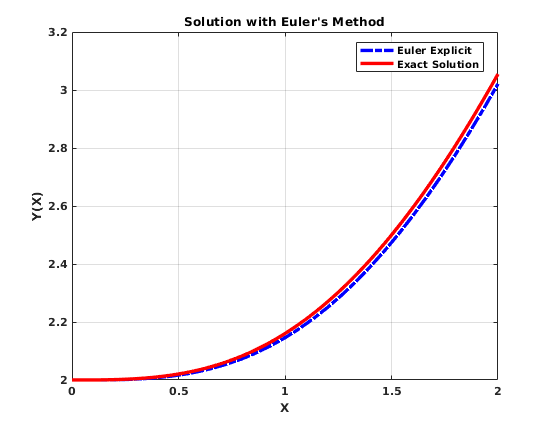
\includegraphics{lec23n-ex1-plot.png}
\caption{Approximate solution of example problem using Euler's explicit method with $N=30$.}
\label{fig:lec23n-ex1-plot}
\end{marginfigure}
A plot of the numeric solution along with the exact solution is shown in Figure \ref{fig:lec23n-ex1-plot}. The numeric solution clearly has errors which, of course, we can reduce if we increase $N$.  The convergence behavior of Euler's explicit method is shown in Figure \ref{fig:lec23n-ex1-converge}.
\begin{marginfigure}[-0.20cm]
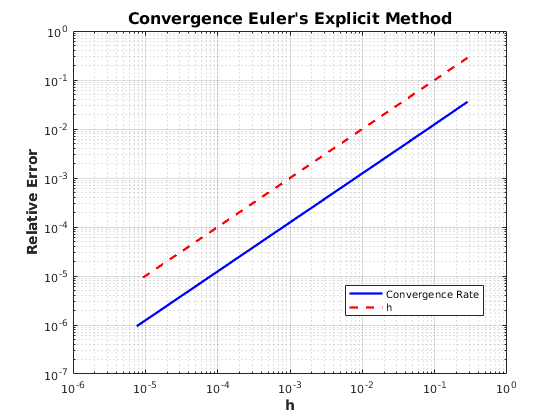
\includegraphics{lec23n-ex1-converge.png}
\caption{Convergence behavior of Euler's explicit method for example problem.}
\label{fig:lec23n-ex1-converge}
\end{marginfigure}

\subsection{Stiff Equations}

\newthought{One disadvantage} of Euler's explicit method for solving IVPs is that for some problems local truncation error, instead of building up steadily, amplify exponentially and the solution ``blows up.''  As an example, consider the following IVP:

\begin{equation}
y^{\prime} = -100[y-\cos{(x)}]- \sin{(x)}, \ \ y(1) = 1, \ \ 0<x<2
\label{eq:lec23n-stiff-ivp}
\end{equation}
The reader is encouraged to verify that the exact solution to this problem is $y^{\star}(x)=cos{(x)}$.  If we discretize the domain into $N=95$ intervals and solve using Euler's explicit method, we get the result shown in Figure \ref{fig:lec23n-ex1-unstable}.
\begin{marginfigure}
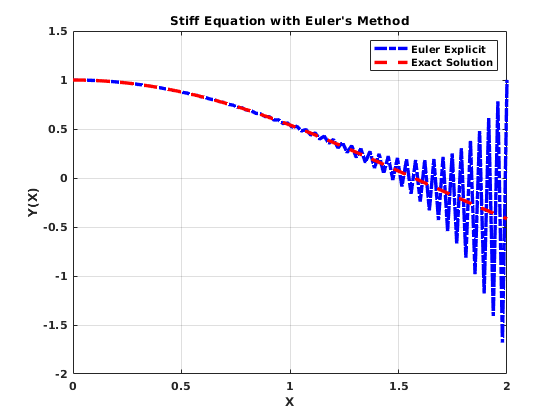
\includegraphics{lec23n-ex1-unstable.png}
\caption{Result of attempting to solve a ``stiff'' differential equation with Euler's explicit method, $N=95$.}
\label{fig:lec23n-ex1-unstable}
\end{marginfigure}
You should look at that figure and recognize that whatever is going wrong, it is more than just the accumulation of local truncation error, but instead signs of incipient instability.  If you reduce $N$ further the numeric result blows up and produces a meaningless result.

The example given in Equation \ref{eq:lec23n-stiff-ivp} is referred to as a ``stiff'' differential equation.  Even though the actual solution is quite smooth, a large number of intervals is required in order to obtain a reasonable numeric solution.  Often it is the case, as it is now, that we can address the stiffness problem by simply increasing $N$ and thereby reducing our step size.  Eventually a threshold is passed where the numeric solution is stable and converges as expected.  In some cases, however, evaluating $f(x,y)$ is computationally expensive and ``simply'' reducing the step size has unacceptable costs.  A conceptually simple change to the algorithm can fix this problem.

\section{Euler's Implicit Method for 1\textsuperscript{st}-Order IVPs}
This method relies on the same theoretical development as the explicit Euler method.  The difference is that, when we solve for $y_{i+1}$, we will use $f(x_{i+1},y_{i+1})$:

\vspace{0.2cm}

\noindent\textbf{Algorithm:}
\begin{enumerate}
\item Discretize the independent variable, $x \in [a,b]$ into $N$ intervals of equal size: $h = (x_{i+1}-x_i) = \frac{b-a}{N}$.
\item Set $y(x_0) = y_0$ where both $x_0$ and $y_0$ are given in the problem statement.
\item Set $x_{i+1} = x_i + h$
\item Evaluate: $y_{i+1} = y_i + hf(x_{i+1},y_{i+1})$
\item Repeat steps 3 and 4, $N$ times.
\end{enumerate}
Note that step 4 of the algorithm requires solving a nonlinear equation (or system of equations).  We have studied methods of solving nonlinear equations previously in this course and we know it is not a trivial problem.  Also, this method is still only 1\textsuperscript{st}-order convergent like its explicit sibling.  The main benefit is that this algorithm will maintain stability even for stiff problems like the last example.

A straight-forward MATLAB implementation is provided in the listing below.
\marginnote{

\vspace{5.5cm}

\ref{lst:ann23n-5} Create an \lstinline[style=myMatlab]{options} structure that will suppress extraneous output of \lstinline[style=myMatlab]{fsolve}.

\vspace{0.5cm}

\ref{lst:ann23n-6} Call \lstinline[style=myMatlab]{fsolve} to find \lstinline[style=myMatlab]{y_ns(t+1)}.
}
\begin{lstlisting}[style=myMatlab,name=lec23n-ex2]
clear
clc
close 'all'

%% Set up the Problem
f_stiff = @(x,y) -100*(y-cos(x))-sin(x);
f_stiff_exact = @(x,y) cos(x);

N = 10
x = linspace(xMin,xMax,N+1);
y_ns = nan(1,N+1);
y_ns(1) = 1;
h = x(2)-x(1);

%% Solve using Implicit Euler's Method
options = optimoptions('fsolve','Display','none'); /*!\annotation{lst:ann23n-5}!*/
for t = 1:N-1
   fe_fun = @(y) y - y_ns(t) - f_stiff(x(t+1),y)*h;
   y_ns(t+1) = fsolve(fe_fun,y_ns(t),options); /*!\annotation{lst:ann23n-6}!*/
end

%% Plot the result
plot(x,y_ns,'-.b',...
    x_gold,f_stiff_exact(x_gold),'--r',...
    'linewidth',3);
title("Stiff Equation with Euler's Method",'fontsize',14,...
    'fontweight','bold');
xlabel('X','fontsize',12,'fontweight','bold');
grid on;
set(gca,'fontsize',10,'fontweight','bold');
ylabel('Y(X)','FontSize',12,'FontWeight','bold');
grid on;
set(gca,'fontsize',10,'fontweight','bold');
legend('Euler Implicit','Exact Solution');
\end{lstlisting}
\begin{marginfigure}
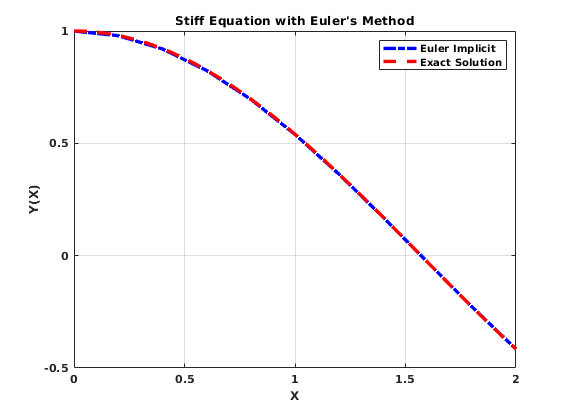
\includegraphics{lec23n-ex2-implicit.png}
\caption{Solution of a stiff IVP with Euler's implicit method with $N=10$.}
\label{fig:lec23n-ex2-implicit}
\end{marginfigure}
The resulting solution is shown in Figure \ref{fig:lec23n-ex2-implicit}.  The performance trade-offs are hard to measure in general. Depending on how many evaluations of $f(x,y)$ are required to solve the nonlinear equations and depending on how stiff the equation is, implicit Euler's method may be less attractive than simply increasing $N$ and trying again with Euler's explicit method.  This trade-off will be different for each problem.

\section{Modified Euler's Method}

Whether you are using the implicit or explicit version of Euler's method, they both exhibit 1\textsuperscript{st}-order convergence which is slow.  Can we do better?  The answer is: of course.  The main assumption in Euler's method is that the slope remains constant throughout each interval.  This is the major source of error and the modified Euler's method partially corrects for this error.

\vspace{0.2cm}

\noindent\textbf{Algorithm:}
\begin{enumerate}
\item Discretize the independent variable, $x \in [a,b]$ into $N$ intervals of equal size: $h = (x_{i+1}-x_i) = \frac{b-a}{N}$.
\item Set $y(x_0) = y_0$ where both $x_0$ and $y_0$ are given in the problem statement.
\item Set $x_{i+1} = x_i + h$
\item Calculate $f(x_i,y_i)$
\item Estimate $y_{i+1}$ using Euler's explicit method: $y^{\text{EE}}_{i+1} = y_i + hf(x_{i},y_{i})$
\item Calculate $f(x_{i+1},y^{\text{EE}}_{i+1})$
\item Find better estimate of $y_{i+1}$ by averaging the two slopes:
\begin{equation*}
y_{i+1} = y_i + \frac{f(x_i,y_i) + f(x_{i+1},y^{\text{EE}}_{i+1})}{2}h
\end{equation*}
\item Repeat steps 3 through 7, $N$ times.
\end{enumerate}
One can show that this algorithm reduces local truncation error to $\mathcal{O}(h^3)$ and the corresponding global truncation error is $\mathcal{O}(h^2)$, thereby obtaining quadratic convergence. The listing below shows a MATLAB implementation of steps 3 through 7 and Figure \ref{fig:lec23n-ex1-modified-convergence} shows the 2\textsuperscript{nd}-order convergence behavior.
\begin{marginfigure}
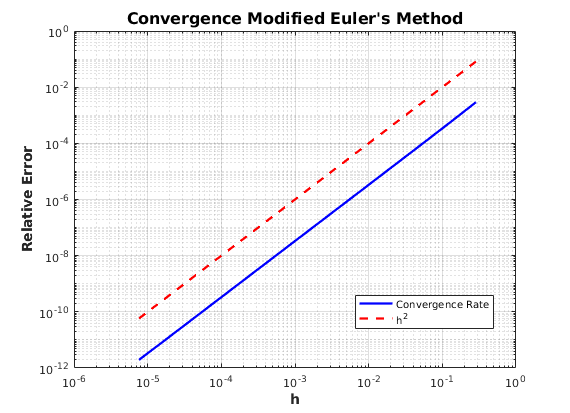
\includegraphics{lec23n-ex1-modified-convergence.png}
\caption{Quadratic convergence of the modified Euler method.}
\label{fig:lec23n-ex1-modified-convergence}
\end{marginfigure}
\begin{lstlisting}[style=myMatlab,name=lec23n-modified]
for t = 1:N
   f_xy = f(x(t),y_ns(t));
   % initial Euler step
   y_ns_EU = y_ns(t) + f_xy*h;
   
   % Apply Mod Euler
   y_ns(t+1) = y_ns(t) + ...
       (f_xy + f(x(t+1),y_ns_EU))*h/2;   
end
\end{lstlisting}








